\chapter{Rotation}
\graphicspath{{../../img/}}


In this lecture, we will discuss how to handle orientation. Robots are typically rigid bodies, that have position and orientation. Positions are simply $x,y, z$ coordinates but rotation is more complex. We will then discuss how we can model the motion and sensing of a robot and bring it back to the optimization theory we discussed. Hence, we have to be able to optimise over position and rotation.

We consider two frames - the world or the map $\{W\}$ and the body reference frame $\{B\}$, for the robot itself. Since the robot remains the same, we can specify the motion of one point $p(t) \in R^3$ and three coordinate axes $r_1(t), r_2(t), r_3(t)$, attached to that point.

\begin{figure}[h]\centering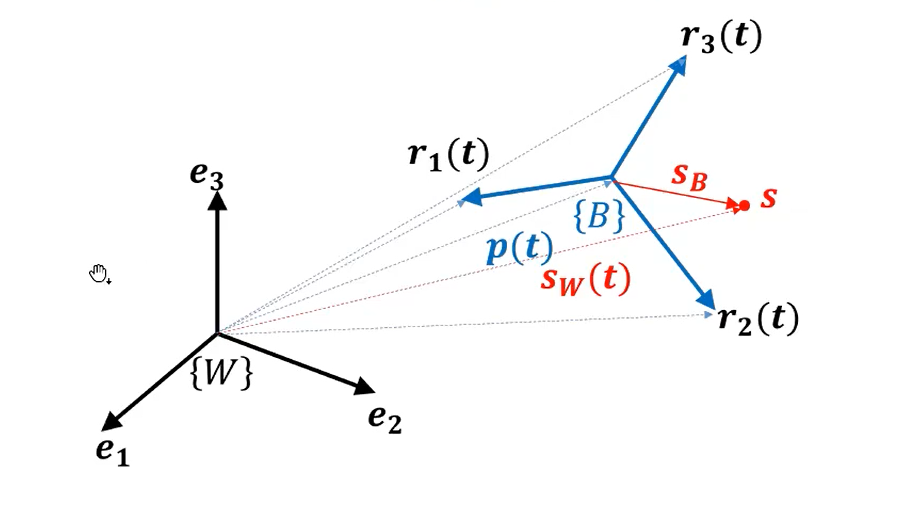
\includegraphics[width=12cm]{img/j_1.png}\end{figure}

In the above figure, we can see the black axes as the world frame, and the blue lines as the body frame. The point $s$ will have constant coordinates with respect to the body frame (it is some point on the robot), but different coordinates in the world frame (since the body is constantly moving). Alternatively,

A point $s$ on the rigid body has fixed coordinates $s_B\in R^3$ in the body frame $\{B\}$ but time-varying coordinates $s_w(t)\in R^3$ in $\{W\}$.

\textbf{Pose}

The pose $T(t)\in SE(3)$ of a rigid body reference frame $\{B\}$ at time $t$ in a fixed world frame $\{W\}$ is determined by:

\begin{enumerate}
    \item The position $p(t)\in R^3$ of $\{B\}$ relative to $\{W\}$.
    \item The orientiation $R(t) \in SO(3)$ of $\frame{B}$ relative to $\frame{W}$, determined by the 3 coordinate axes $r_1(t), r_2(t), r_3(t)$.
\end{enumerate}

Now, how do we describe the space of orientations of orientations $SO(3)$ and the space of poses $SE(3)$.

\section{Special Euclidian Group}

Rigid body motion is described by a sequence of functions that describe how the coordinates of 3-D points on the object change with time.

Rigid body motion preserves distances (vector norms) and does not allow reflection of the coordinate system (vector cross products).

For instance, the distance between our eyes should not change when we move around. Further, it shouldn't be possible to get a mirror image of a body when it moves.

The \textbf{Euclidian Group} $E(3)$ is a set of functions $g: R^3\to R^3$ that preserves the norm of any two vectors.

The \textbf{Special Euclidian Group} $SE(3)$ is a set of functions $g: R^3\to R^3$ that preserve the norm and the cross product of any two vectors.

\begin{enumerate}
    \item Norm: $\norm{g_*(u) - g_*(v)} = \norm{v-u}, \forall u, v \in R^3$.
    \item Cross product: $g_*(u) \times g_*(v) = g_*(u\times v), \forall u, v \in R^3$
\end{enumerate}

where $g_*(x) := g(x) - g(0)$.

\textbf{Corollary:} $SE(3)$ elements $g$ also preserve:

\begin{enumerate}
    \item Angle: $u^Tv = \frac{1}{4} (\norm{u + v}^2 - \norm{u-v}^2) \implies u^Tv = g_*(u)^T g_*(v), \forall u, v \in R^3$.
    \item Volume: $\forall u, v, w \in R^3, g_*(u)^T(g_*(v)\times g_*(w))=u^T(v\times w)$
\end{enumerate}

Pure rotation is a special case of rigid body motion. The orientation of the body frame $\frame{B}$ in the world frame $\frame{W}$ is determined by the coordinates of the three orthogonal vectors $r_1 = g(e_1), r_2 = g(e_2), r_3 = g(e_3)$, transformed from $\frame{B}$ to $\frame{W}$.

The vectors organized in a $3\times 3$ matrix specify the orientation of $\frame{B}$ in $\frame{W}$:

\begin{equation*}
    {}_{\frame{W}}R_{\frame{B}} = \begin{bmatrix}
        r_1 & r_2 & r_3
    \end{bmatrix} \in \R^{3\times 3}
\end{equation*}

Consider a point with coordinates $s_B\in R^3$ in $\frame{B}$. Its coordiantes $s_W$ in $\frame{W}$ are:

\begin{equation*}
    \begin{split}
        s_W &= [s_B]_1r_1 + [s_B]_2r_2 + [s_B]_3r_3 \\
        &= Rs_B
    \end{split}
\end{equation*}

\begin{figure}[h]\centering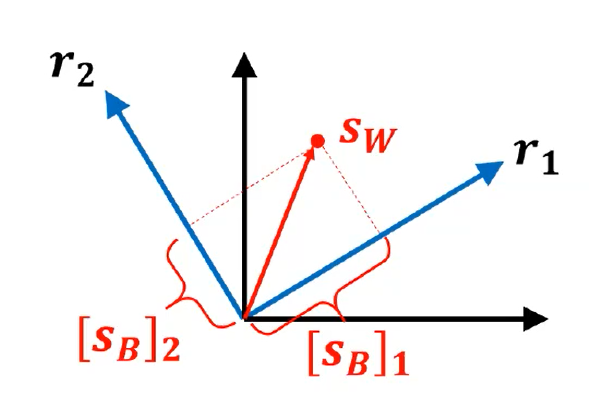
\includegraphics[width=7cm]{img/j_3_2.png}\end{figure}

\red{Not sure if this is correct} This is because the transformation from the body frame to world frame is the same as the position of the body frame in the world frame.

The rotation transformation $g$ from $\frame{B}$ to $\frame{W}$ is:

\begin{equation*}
    g(s) = Rs
\end{equation*}

\section{Special Orthogonal Group $SO(3)$}

$r_1, r_2, r_3$ from an orthonormal basis: $r_i^Tr_j = 1$ (when $i=j$), else $0$.

Since $r_1, r_2, r_3$ form an orthonormal basis, the inverse of R is its transpose $R^TR=I$ and $R^{-1} = R^T$.

\begin{figure}[h]\centering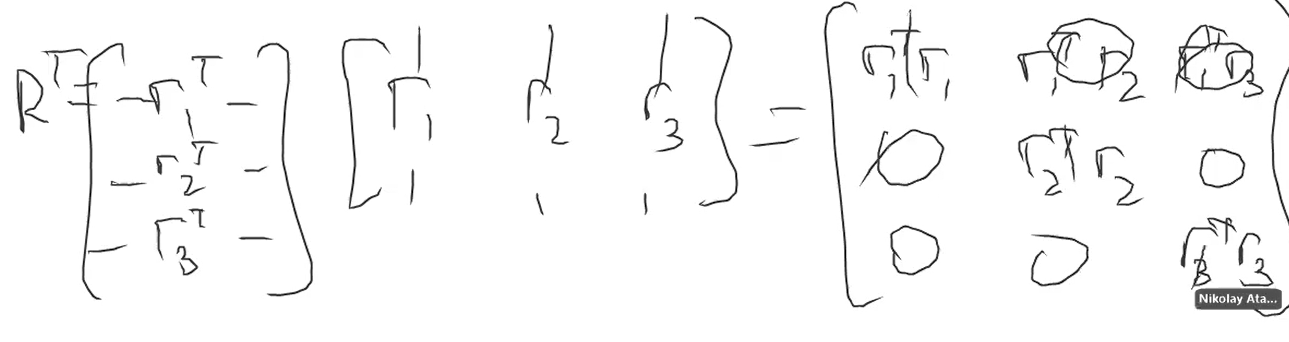
\includegraphics[width=12cm]{img/j_3_3.png}\caption{A quick illustration to see why $R^TR=I$}\end{figure}

$R$ belongs to the orthogonal group:

\begin{equation*}
    O(3): = \{ R\in \R^{3\times 3} | R^TR = RR^T = I\}
\end{equation*}

Distance preserving: Let's look at -

\begin{equation*}
    \begin{split}
        \norm{Rx - Ry}^2 = \norm{R(x - y)}^2 = (x - y)^TR^TR(x - y) = (x - y)^T(x - y) = \norm{x - y}^2
    \end{split}
\end{equation*}


Reflections are not allowed since $\text{det}(R) = r_1^T(r_2\times r_3) = 1$:

\begin{equation*}
    R(x\times y) = R(x\times (R^TRy)) = (R\hat{x}R^T)Ry = \frac{1}{det(R)}(Rx)\times (Ry)
\end{equation*}

Hence, we can say that $R$ belongs to the special orthogonal group:

\begin{equation*}
    SO(3) : = \{ R\in \R^{3\times 3} | R^TR = I, det(R) = 1\}
\end{equation*}

\section{2D Rotations}

\subsection{Angles}

In two dimensions, we can just use an angle around Z axis to represent rotation.

\begin{figure}[h]\centering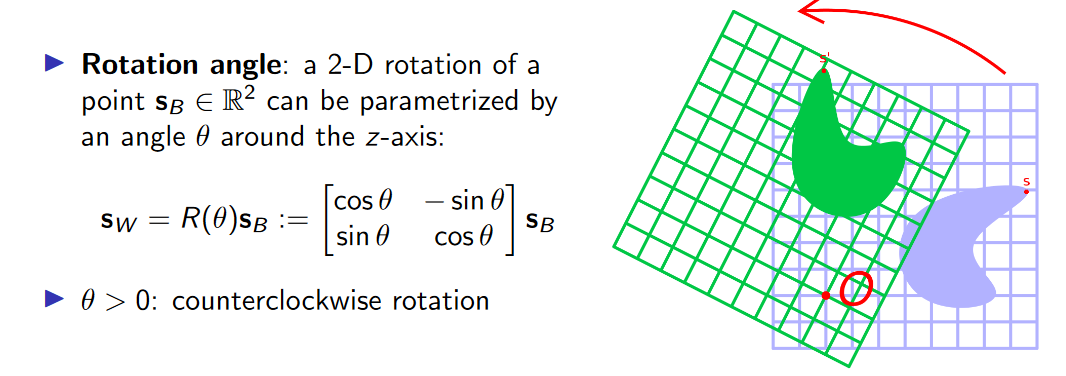
\includegraphics[width=12cm]{img/j_3_4.png}\end{figure}

The angle works out this way because of right hand thumb rule (fingers curl in direction of rotation - axis coincides with thumb)

The matrix values can be calculated by simply making the columns the positions of the X and Y axis after rotation.

\subsection{Unit-norm Complex Number}

We can represent a rotation by a complex number, something like $e^{i\theta}$, which can be expanded by euler's formula:

\begin{equation*}
    e^{i\theta} = \cos\theta + i\sin\theta
\end{equation*}

Or, if we have a 2D rotation of $[s_B]_1 + i[s_B]_2\in \C$

\begin{figure}[h]\centering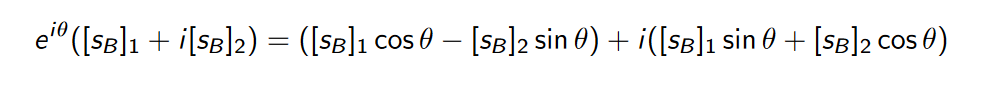
\includegraphics[width=12cm]{img/j_3_5.png}\end{figure}

We'll revisit this in the 3D scenario.

\section{3D Rotation}

\textbf{Euler Angles}

This is our 3D extension of the 2D angle representation. When in 2D, we had an angle around one axis, in 3D, we have it about 3 different axes.

Or, Euler angles: an extension of the rotation angle parametrization of 2-D rotations that specifies rotation angles around the three principal axes.

\textbf{Axis Angle}

An extension of the rotation angle parametrization of 2-D rotations that allows the axis of rotation to be chosen freely instead of being a fixed principal axis.

\textbf{Unit Quaternion}

An extension of the unit-norm complex number parametrization of 2-D rotations.

\subsection{Euler Angles}

This uses three angles to specify rotation around three principal axes.

There are 24 different ways to apply these rotations - depending on the order, which axes we come back to, whether we rotate around original axes, or we keep using the updated one.

\begin{enumerate}
    \item Extrinsic axes: The rotation axes remain static
    \item Intrinsic Axes: THe rotation axes move with the rotations.
    \item Further, there are two groups that they can be divided into:
    \begin{enumerate}
        \item Euler angles: Rotat ion about one axis, then a second, and then the first
        \item Tait-bryan Angles: Rotation about all three axes.
    \end{enumerate}
\end{enumerate}

The Euler and Tait-Bryan Angles each have 6 possible choices for each of the extrinsic/intrinsic groups leading to 2 * 2 * 6 = 24 possible conventions to specify a rotation sequence with three given angles.

This is a mess - too many options!

Hence, when we deal with euler, we must specify rotations explicitly:

\begin{enumerate}
    \item r (rotating = intrinsic) or s (static = extrinsic)
    \item xyz or zyx or zxz, etc. (order of rotation axes)
\end{enumerate}

The most widely used one is row-pitch-yaw convention

\subsubsection{Row-Pitch-Yaw Convention}

\begin{figure}[h]\centering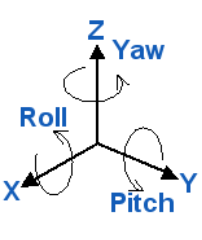
\includegraphics[width=3cm]{img/j_3_6.png}\end{figure}

Roll ($\phi$), pitch ($\theta$), yaw ($\psi$) angles are used in aerospace engineering to specify rotation of an aircraft around the x, y, and z axes, respectively.

Now, elementary rotations can be represented as follows:

\begin{figure}[h]\centering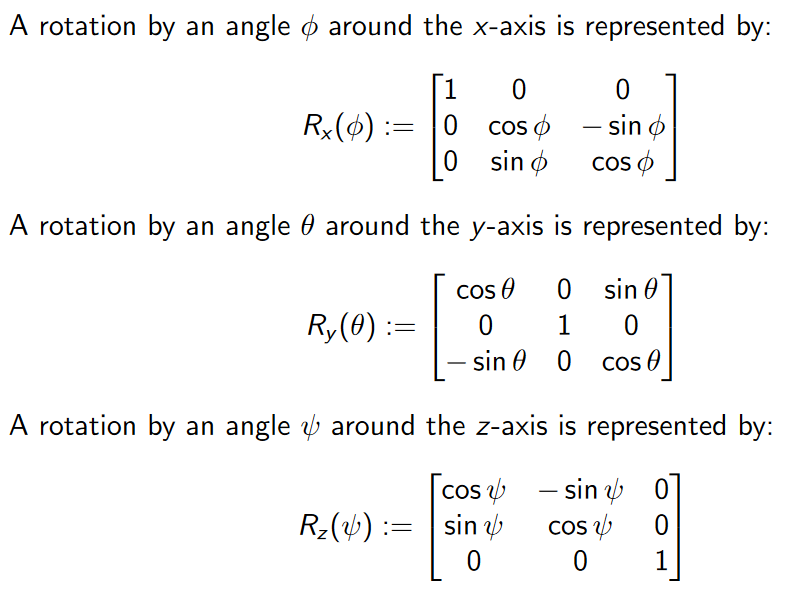
\includegraphics[width=8cm]{img/j_3_7.png}\end{figure}

If we are given some information about the roll, pitch, yaw, we can compute the $R$ matrix as follows: \clearpage

\begin{figure}[h]\centering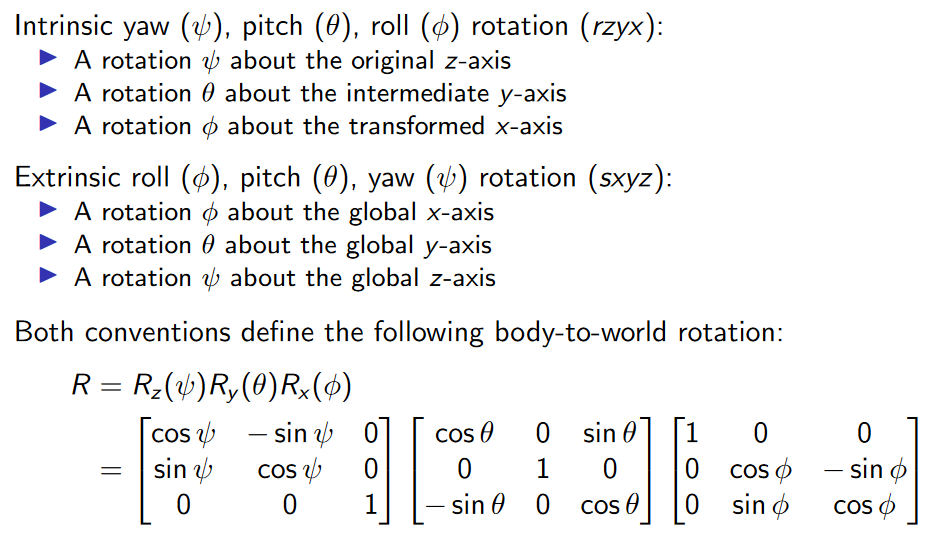
\includegraphics[width=10cm]{img/j_3_8.png}\end{figure}

\subsubsection{Gimbal Lock}

Ideally, with three variables, and three degrees of freedom, we should be able to represent all rotations but this is not true. This is gimbal lock. Alternatively, angle paramterizations are not one-to-one.

Example: if the pitch becomes $\theta = 90\deg$, the roll and yaw become associated with the same degree of freedom and cannot be uniquely determined.

\begin{figure}[h]\centering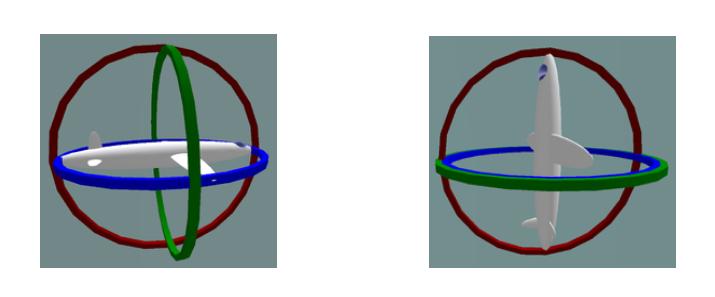
\includegraphics[width=12cm]{img/j_3_9.png}\caption{Look at what happens after the pitch - two axes align and we can't distinguish between roll and yaw.}\end{figure}

Hence, two big problems with euler - it's confusing and gimbal lock.

\subsection{Axis Angle Representation}

\subsubsection*{Cross Product Review}

\begin{figure}[h]\centering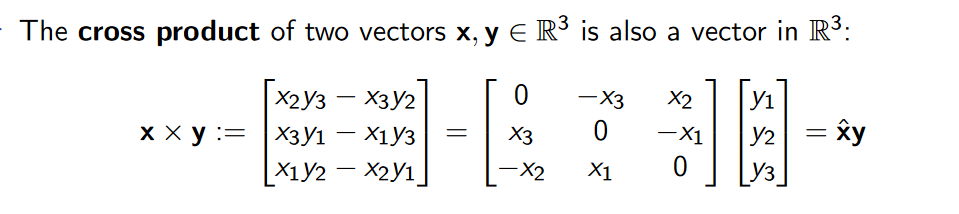
\includegraphics[width=12cm]{img/j_3_10.png}\end{figure}

$\hat{x}$ is the skew symmetric matrix used to represent the $x$ that is used for cross product. It is also called the \b{hat map}.

\begin{figure}[h]\centering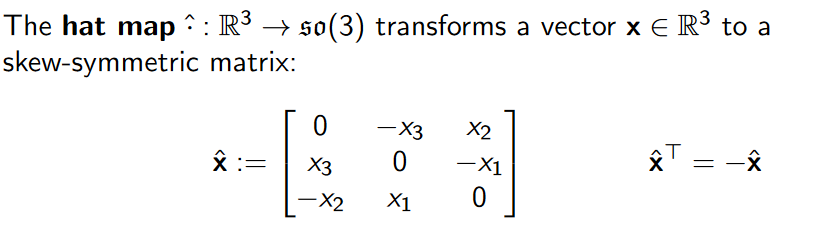
\includegraphics[width=10cm]{img/j_3_11.png}\end{figure}

The vector space $\R^3$ and the space of skew-symmetric $3\times3 $ matrices $so(3)$ are isomorphic, i.e., there exists a one-to-one map (the hat map) that preserves their structure.

The \b{vee map} (v because its the upside down version of the hat) simply obtains $x$ back from the skew-symmetric matrix $\hat{x}$.

\begin{figure}[h]\centering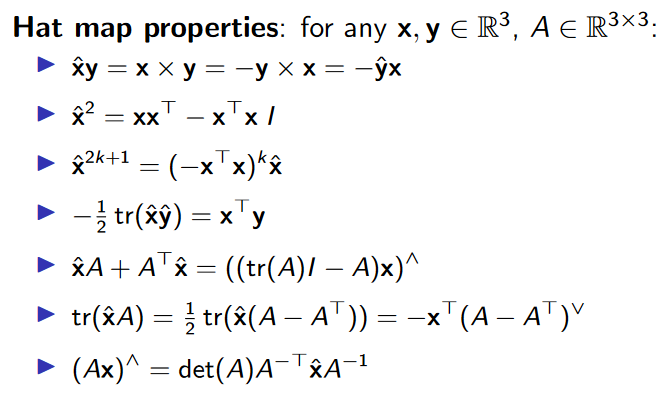
\includegraphics[width=10cm]{img/j_3_12.png}\end{figure}

Coming back to axis-angle. 

Let's assume that we have a stick on a cylinder that is rotating about the cylinder. Let us consider a point $s$ at the end of this stick.

\begin{figure}[h]\centering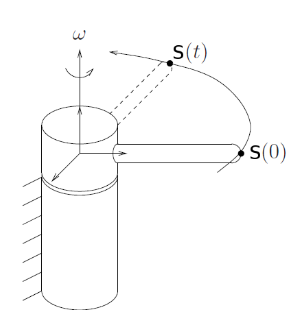
\includegraphics[width=5cm]{img/j_3_13.png}\end{figure}

Let the point have a constant unit velocity, such that:

\begin{equation*}
    \dot{s}(t) = \eta \times s(t) = \hat{\eta} s(t)
\end{equation*}

Now, $s(t) = R_z(t)s(0)$.

This is simply a linear time-invariant system of ordinary differential equations determined by the skew symmetric matrix $\hat{\eta}$. The solution for this can be written as (this is a standard solution):

\begin{equation*}
    s(t) = \text{exp}(\hat{\eta t}s(0))
\end{equation*}

\begin{equation*}
    s(t) = R_n(t)s(0)
\end{equation*}

We can just replace the $t$ with $\theta$,

\begin{equation*}
    s(t) = \text{exp}(\hat{\eta \theta}s(0))
\end{equation*}

\begin{equation*}
    s(t) = R_n(\theta)s(0)
\end{equation*}

This is the exponential map:

\begin{figure}[h]\centering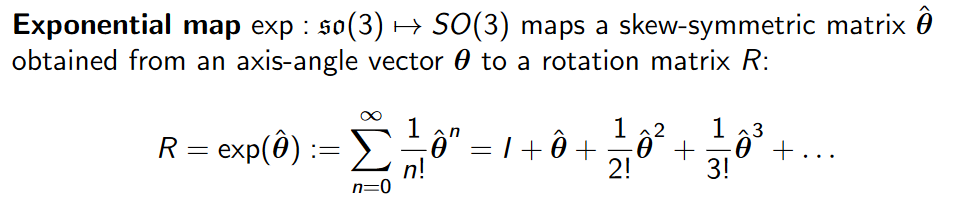
\includegraphics[width=10cm]{img/j_3_14.png}\end{figure}

\red{Look at Hao Su's description of axis angle and the conversions there}.

The skwigly so is simply the set of skew symmetric matrices. The exponential map maps every skew symmetric matix to a special orthogonal group rotation.

$\text{exp}$ is not the same as taking exponential of every element, but rather:

\begin{equation*}
    \text{exp}(A) = I + A + \frac{1}{2}AA + \frac{1}{3!}AAA
\end{equation*}

\begin{figure}[h]\centering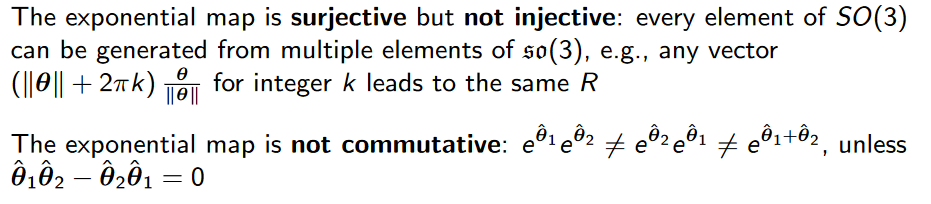
\includegraphics[width=12cm]{img/j_3_15.png}\end{figure}

\textbf{Rodriguez Formula}

It is the closed form expression for the exponential map from the skew symmetric space to special orthogonal group:

\begin{figure}[h]\centering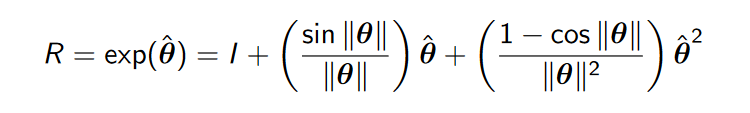
\includegraphics[width=8cm]{img/j_3_16.png}\end{figure}

An important property to derive this is that $\hat{x}\hat{x} = xx^T - x^TxI$. Further, any odd power of $\hat{x}$ can be written as some product of $x$. 

\clearpage

\begin{figure}[h]\centering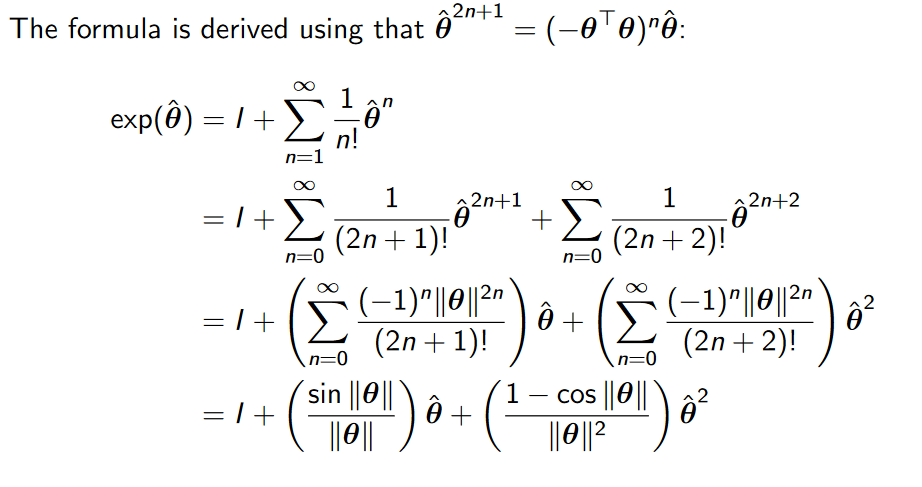
\includegraphics[width=10cm]{img/j_3_17.png}\end{figure}

In the above equation, we split the infinite sum into odd powers and even powers respectively (look at the superscript). 

Then, we subtitute the odd power of $\hat{\theta}$ with the equation that expresses it as a product of $\hat{\theta}$. 

The final line is simply the expansion of $\sin$ and $\cos$. 

\b{Why do we need it?}

This is faster, closed form. Practically, doesn't matter but this is better obviously.

\b{Log Map}

There is a log map that simply inverts the exponential - it goes from SO group to the skew symmetric group.

\begin{figure}[h]\centering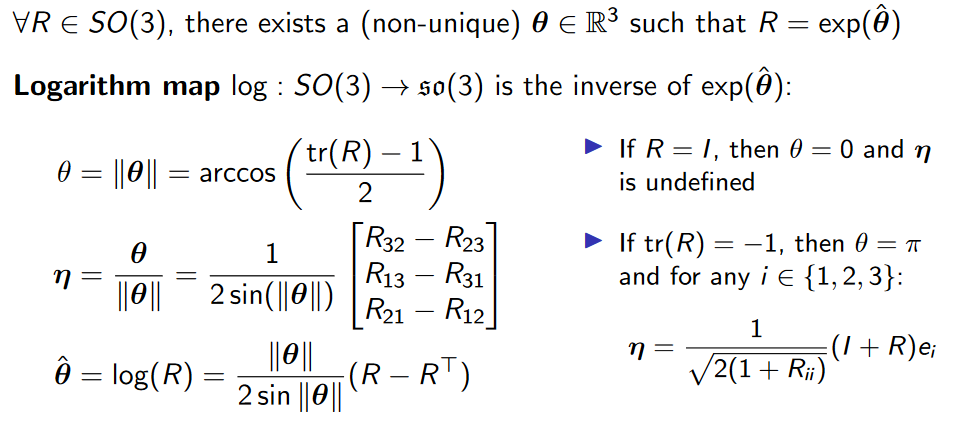
\includegraphics[width=12cm]{img/j_3_18.png}\caption{All this is derived from the rodriguez formula}\end{figure}

The log map is not unique - so it's not a true inverse. $R$ is not truly invertible.

The matrix exponential ``integrates'' $\hat{\theta} \in se(3)$ for one second; the matrix logarithm ``differentiates'' $R \in SO(3)$ to obtain $\hat{\theta} \in se(3)$.

\subsection{Quaternion}

We now look for a representation that doesn't have singularity. Quaternions are a solution for this, and are an extension of the complex number idea that we had disucssed earlier. 

\begin{figure}[h]\centering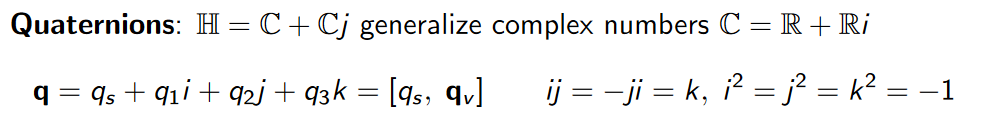
\includegraphics[width=12cm]{img/j_3_19.png}\end{figure}

Here, $\H$ is the quaternion space. $\H_*$ is the space of unit-norm quaternions:

\begin{equation*}
    \H_* := {q\in \H | q_s^2 + q_v^Tq_v = 1}
\end{equation*}

A vector with a unit-norm is essentially a sphere, so quaternions are 4-D spheres. The surface of the sphere is 3-D dimensional. Hence, every surface of the sphere is a rotation matrix. More accurately, only half of the space is a rotation matrix.

\begin{figure}[h]\centering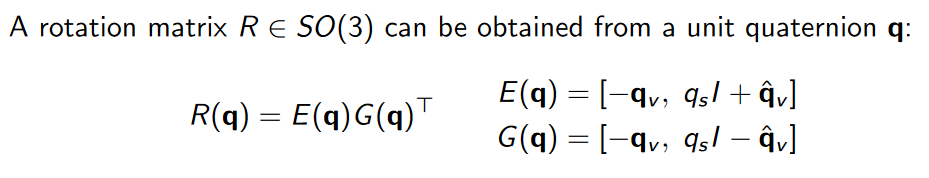
\includegraphics[width=12cm]{img/j_3_20.png}\end{figure}

The fact that only half the sphere is relevant is called double covering of quaternions - $R(q) = R(-q)$.

We can also convert quaternion from axis-angle representation.

\begin{figure}[h]\centering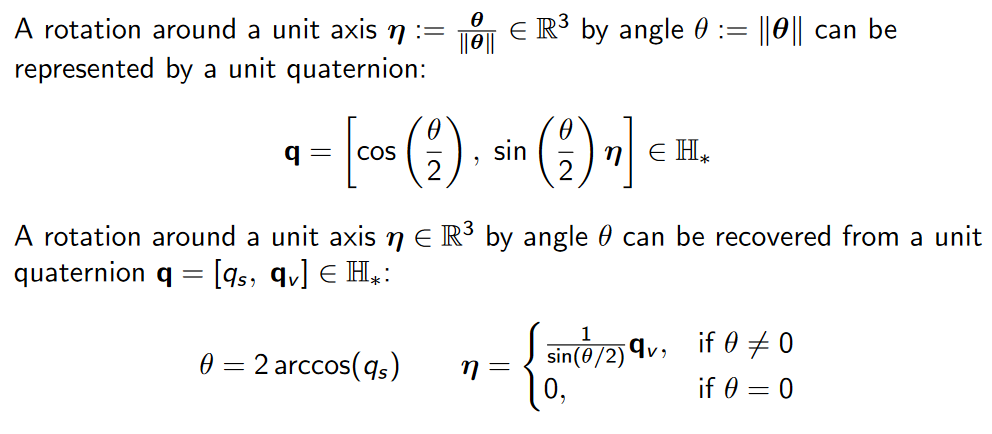
\includegraphics[width=10cm]{img/j_3_21.png}\end{figure}

\clearpage

\textbf{Quaternion Operations}

\begin{figure}[h]\centering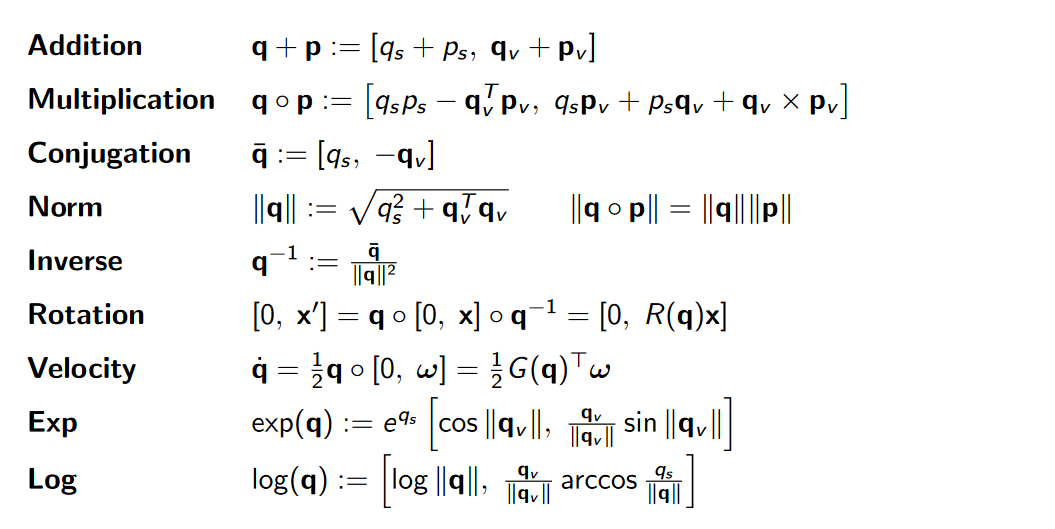
\includegraphics[width=12cm]{img/j_3_22.png}\end{figure}


